\documentclass{beamer}
\usepackage{beamerthemesplit}
\usetheme{innoQ}
\setbeamertemplate{navigation symbols}{}
% \beamersetuncovermixins{\opaqueness<1>{15}}{\opaqueness<2->{10}}
\def\pdfshellescape{1}
\usetikzlibrary{calc}
% \usepackage[utf8]{inputenc}
\usepackage[T1]{fontenc}
\usepackage{textcomp}
% \usepackage{listings}
\usepackage{minted}
\usepackage{graphicx}
\usepackage{wasysym}
\usepackage{url}        % for displaying URLs correctly
\usepackage{soul}       % for \caps
% \usepackage{ulem}       % for \sout
\usepackage{hyperref}
\usepackage[ngerman]{babel}
\usepackage{pifont}

\date{Booster 2013, Bergen, NO \\ 2013-03-14}
\author{FND \& wvk, innoQ Deutschland GmbH}

\title{ROCA}
\subtitle{Embrace the Web}


% fonts
\RequirePackage{fontspec}
\defaultfontfeatures{Mapping=tex-text}
\setmainfont[BoldFont={MetaOT-Medi}, BoldItalicFont={MetaOT-MediIta}, ItalicFont={MetaOT-NormIta}, SlantedFont={MetaOT-NormIta}, BoldSlantedFont={MetaOT-MediIta}, Ligatures=TeX]{MetaOT-Norm}
\setsansfont[BoldFont={MetaOT-Medi}, BoldItalicFont={MetaOT-MediIta}, ItalicFont={MetaOT-NormIta}, SlantedFont={MetaOT-NormIta}, BoldSlantedFont={MetaOT-MediIta}, Ligatures=TeX]{MetaOT-Norm}

\newfontfamily\metamedifamily[SlantedFont={MetaOT-MediIta}]{MetaOT-Medi}

\begin{document}
  {\usebackgroundtemplate{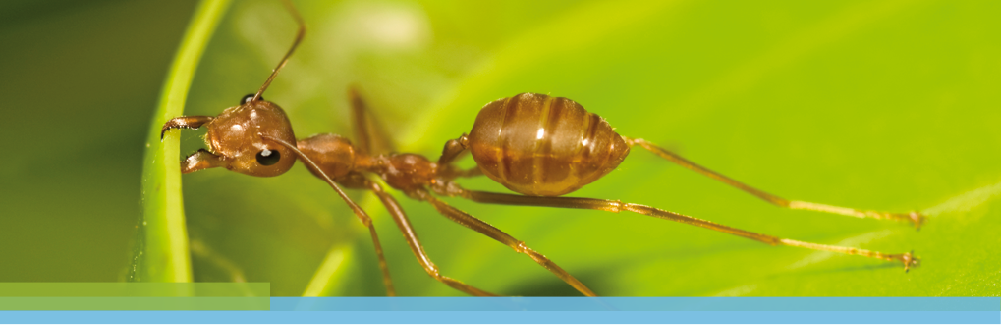
\includegraphics[width=\paperwidth]{images/innoqbg.png}}

  \begin{frame}[plain]
    \titlepage
  \end{frame}
}

\setcounter{tocdepth}{1}

\begin{frame}
  \begin{columns}
    \begin{column}{4.4cm}
      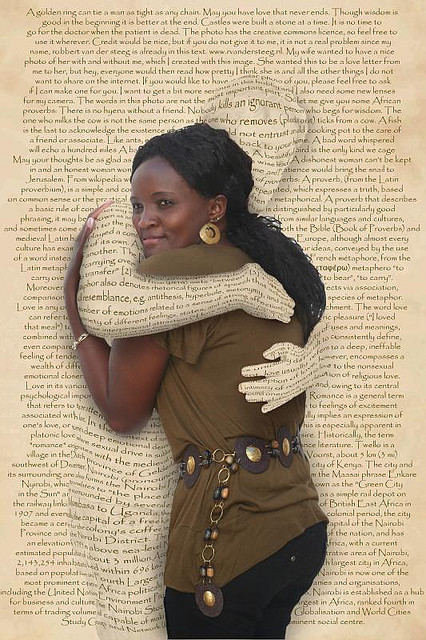
\includegraphics[width=4cm]{images/embrace.jpg}
      \\
      \tiny source: \href{http://www.flickr.com/photos/robbie73/4289385819/}{Robbert van der Steeg}
    \end{column}

    \begin{column}{6.6cm}
      \tableofcontents
    \end{column}
  \end{columns}
\end{frame}

\section{Hej.}

\begin{frame}{\insertsectionhead}
  \begin{itemize}
    \item[FND] Frederik Dohr \\
        recovering SPA enthusiast (\ensuremath{\rightarrow} TiddlyWiki)
    \item[]
    \item[wvk] Willem van Kerkhof \\
        TODO
  \end{itemize}

\end{frame}

\section{What's ROCA?}

{
  \usebackgroundtemplate{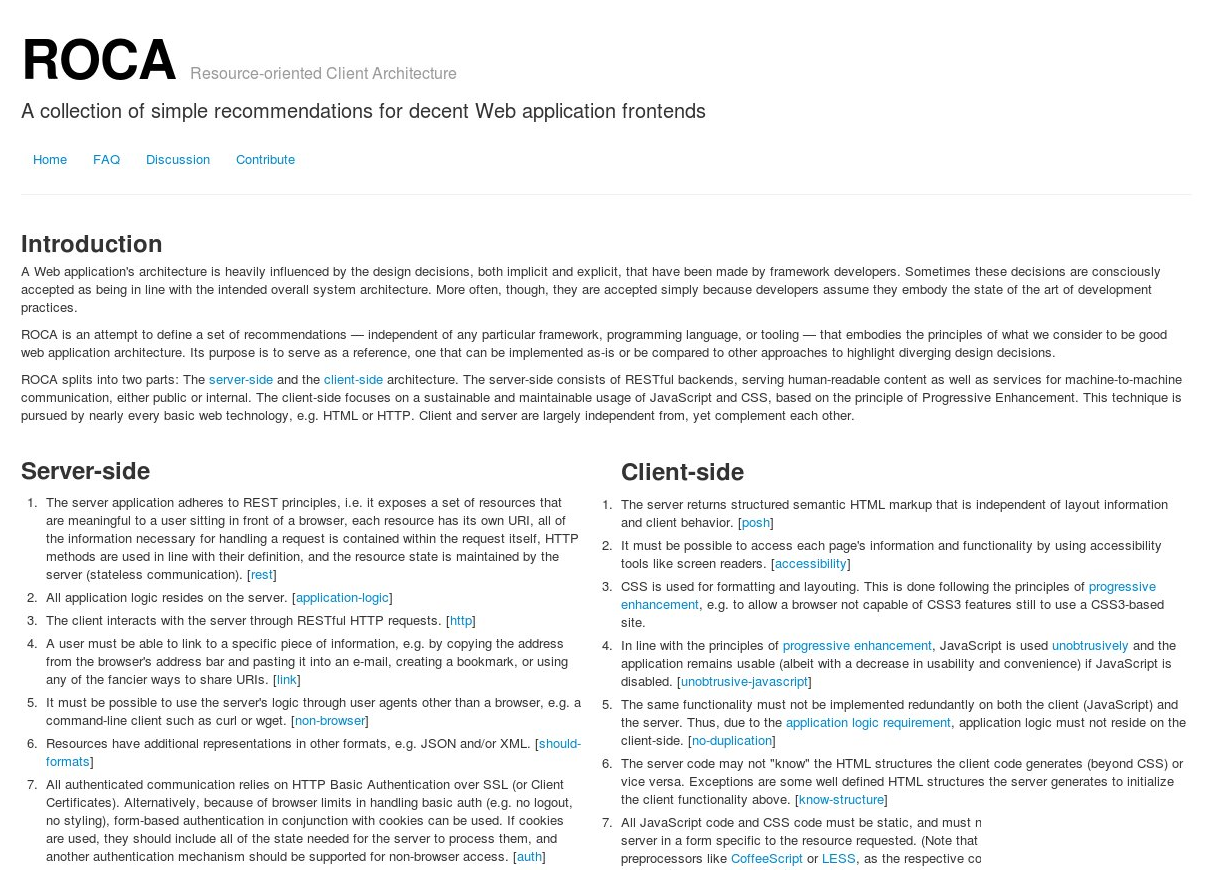
\includegraphics[width=\paperwidth]{images/roca-website.png}}
  \begin{frame}
    \vspace*{-2.5in}
    \href{http://roca-style.org}{roca-style.org}
  \end{frame}
}

\begin{frame}
  \Huge Yet another Manifesto?
\end{frame}

{
  \usebackgroundtemplate{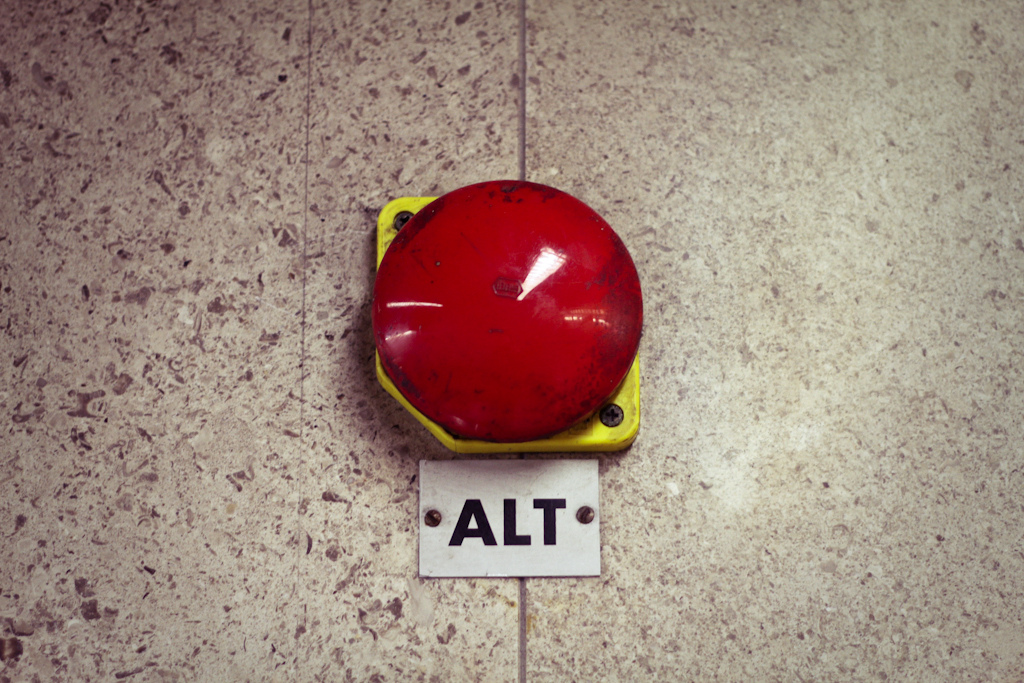
\includegraphics[width=\paperwidth]{images/buzzer.jpg}}
  \begin{frame}
    \vfill
    \vfill
    \vfill
    \vfill
    \vfill
    \vfill
    \vfill
    \vfill
    \vfill
    \vfill
    \textcolor{white}{
      \small source: \href{http://www.flickr.com/photos/sensorsicht/5338348801/}{Hannes Fritz}
    }
  \end{frame}
}

\subsection{MUST criteria}

\begin{frame}{REST}
  The server application adheres to REST principles

  \begin{itemize}
    \item it exposes meaningful resources
    \item each resource has its own URI
    \item all necessary request handling information is contained within the request
    \item HTTP methods are used in line with their definition
    \item resource state is maintained by the server
  \end{itemize}
\end{frame}

\begin{frame}{Application Logic on Server}

  All essential application logic resides on the server.

  \begin{itemize}
    \item a service without business logic is a database.
  \end{itemize}
%   wvk
\end{frame}

\begin{frame}{Non-Browser Clients}

  The server's logic should be accessible to other user clients than a browser,

  \begin{itemize}
    \item crawler, indexer (SEO fo free, yay!)
    \item alternative user agent (curl, text browser, screen reader etc.)
    \item arbitrary unanticipated usage
  \end{itemize}
%   wvk
\end{frame}

\begin{frame}{HTTP}

  Client-Server interaction through RESTful HTTP requests.

  \begin{itemize}
    \item well, just like that. Period.
  \end{itemize}
\end{frame}

\begin{frame}{Links}

  A user must be able to link to a specific piece of information

  \begin{itemize}
    \item e.g. by copying the address from the browser's address bar
    \item pasting it into an e-mail or IM
    \item creating a bookmark
    \item or using any of the fancier ways to share URIs
  \end{itemize}
%   wvk
\end{frame}

%   FND
\begin{frame}{POSH}

  The server returns structured semantic HTML markup, independent of layout information or client behavior.
  \\

  HTML offers 

  \ensuremath{\rightarrow}
  \href{http://codeartisan.blogspot.de/2012/07/using-html-as-media-type-for-your-api.html}{Using HTML as the Media Type for your API}
  \\

  (alternative serializations are encouraged)

\end{frame}

% FND
\begin{frame}{Unobtrusive JavaScript}
  JavaScript is used unobtrusively

  \begin{itemize}
    \item the application remains usable without JavaScript.
    \item a decrease in usability and convenience is OK and expected (B/W-TV vs. HD)
    \item ...as long as core functionality remains available
  \end{itemize}
\end{frame}

\subsection{SHOULD criteria}

\begin{frame}{}
  % Resources have additional representations in other formats, e.g. JSON and/or XML. [should-formats]

  \begin{itemize}
    \item
  \end{itemize}
\end{frame}

\begin{frame}{}
  \begin{itemize}
    \item
  \end{itemize}
\end{frame}


\begin{frame}

% All authenticated communication relies on HTTP Basic Authentication over SSL (or Client Certificates). Alternatively, because of browser limits in handling basic auth (e.g. no logout, no styling), form-based authentication in conjunction with cookies can be used. If cookies are used, they should include all of the state needed for the server to process them, and another authentication mechanism should be supported for non-browser access. [auth]
% Cookies may not be used for purposes other than authentication or user tracking. [cookies]
% There may not be any session state beyond what’s needed for simple algorithmic validation of authentication information. [session]
% The browser controls like the back, forward and refresh buttons must work as expected. I.e. the back button should take the users where they expect to be taken to (the last meaningful resource they worked with). A browser refresh should not cause a re-rendering of the login or home page instead of the page the user was looking at, or a (to the user) unexpected question about wanting to submit the same data again (when the user doesn't recall submitting any data, indicating a mis-use of the POST verb). [browser-controls]

% It must be possible to access each page's information and functionality by using accessibility tools like screen readers. [accessibility]
% CSS is used for formatting and layouting. This is done following the principles of progressive enhancement, e.g. to allow a browser not capable of CSS3 features still to use a CSS3-based site.
% The same functionality must not be implemented redundantly on both the client (JavaScript) and the server. Thus, due to the application logic requirement, application logic must not reside on the client-side. [no-duplication]
% The server code may not "know" the HTML structures the client code generates (beyond CSS) or vice versa. Exceptions are some well defined HTML structures the server generates to initialize the client functionality above. [know-structure]
% All JavaScript code and CSS code must be static, and must not be dynamically generated by the server in a form specific to the resource requested. (Note that this does not prohibit the use of preprocessors like CoffeeScript or LESS, as the respective code is usually pre-compiled as part of the release process.) [static-assets]
% 
% Any dynamic routing or URI state modification triggered by JavaScript on the client side should use the HTML5 History API. [historyapi]
% 

\end{frame}

\section{Quiz Time!}
\begin{frame}
% Cookies may not be used for purposes other than authentication or user tracking. [cookies]


% All authenticated communication relies on HTTP Basic Authentication over SSL (or Client Certificates). Alternatively, because of browser limits in handling basic auth (e.g. no logout, no styling), form-based authentication in conjunction with cookies can be used. If cookies are used, they should include all of the state needed for the server to process them, and another authentication mechanism should be supported for non-browser access. [auth]

% There may not be any session state beyond what’s needed for simple algorithmic validation of authentication information. [session]

% The browser controls like the back, forward and refresh buttons must work as expected. I.e. the back button should take the users where they expect to be taken to (the last meaningful resource they worked with). A browser refresh should not cause a re-rendering of the login or home page instead of the page the user was looking at, or a (to the user) unexpected question about wanting to submit the same data again (when the user doesn't recall submitting any data, indicating a mis-use of the POST verb). [browser-controls]

\end{frame}

\begin{frame}
  Cookies are being used to store form inputs from a previous step.
  \begin{itemize}
    \item[$\square$] \ding{51}
    \item[$\square$] \ding{55}
  \end{itemize}
\end{frame}

\begin{frame}
  When sharing a URL with another user, that user is presented with an empty page.
  [-> session state]
\end{frame}

\begin{frame}
  redirect session data, multi-tab conflicts
\end{frame}

\begin{frame}
  When refreshing the page, the user is taken to the initial entry point.
\end{frame}

\begin{frame}
  After using the browser's back button, the user is presented with an error messsage informing them to use the website's own navigation instead.
\end{frame}

\begin{frame}
  After bookmarking the current page and returning to it later, the user is taken to the website's frontpage.
\end{frame}

\begin{frame}
  ...
\end{frame}

\begin{frame}{Kontakt}
  \begin{columns}
    \column{5cm}
    
\includegraphics[width=4cm]{images/innoQ-Logo-RGB-72dpi.png}
    \vspace{4mm}
    \column{4.5cm}
    \textbf{http://www.innoq.com \\info@innoq.com}
  \end{columns}

  \begin{columns}
    \column{5cm}
      innoQ Deutschland GmbH\\
      Krischerstraße 100\\
      D- Monheim\\
      Tel     +49 \\
      Fax     +49

    \column{5cm}
      innoQ Schweiz GmbH \\
      Gewerbestrasse 11 \\
      CH-6330 Cham \\
      Tel     +41 41 743 01 11
    \end{columns}
  \vspace{10mm}

  \textbf{
    Frederik Dohr      <fnd@innoq.com> \\
    Willem van Kerkhof <wvk@innoq.com>
  }
\end{frame}

\end{document}
